\documentclass[12pt, aspectratio=169]{beamer}
\usepackage{
    hyperref,
    graphicx,
    % enumitem,
    transparent,
    siunitx,
    pgfpages,
    caption,
    booktabs,
    multirow,
    bm,
    standalone,
    tikz,
    comment,
    xcolor,
    svg,
}
\usepackage[hang,flushmargin]{footmisc}
\setbeameroption{hide notes}
% \setbeameroption{show only notes}
\setbeameroption{show notes on second screen}
\setbeamertemplate{note page}[plain]
\setbeamercovered{transparent}

% get rid of junk
\usetheme{default}
\usecolortheme{orchid}
\beamertemplatenavigationsymbolsempty
\hypersetup{pdfpagemode=UseNone} % don't show bookmarks on initial view

% named colors
\definecolor{offwhite}{RGB}{249,242,215}
\definecolor{foreground}{RGB}{255,255,255}
\definecolor{background}{RGB}{24,24,24}
\definecolor{title}{RGB}{107,174,214}
\definecolor{gray}{RGB}{155,155,155}
\definecolor{subtitle}{RGB}{102,255,204}
\definecolor{hilight}{RGB}{102,255,204}
\definecolor{vhilight}{RGB}{255,111,207}
\definecolor{lolight}{RGB}{155,155,155}
%\definecolor{green}{RGB}{125,250,125}

% use those colors
\setbeamercolor{titlelike}{fg=title}
\setbeamercolor{subtitle}{fg=subtitle}
\setbeamercolor{institute}{fg=gray}
\setbeamercolor{normal text}{fg=foreground,bg=background}
\setbeamercolor{item}{fg=foreground} % color of bullets
\setbeamercolor{subitem}{fg=foreground}
\setbeamercolor{itemize/enumerate subbody}{fg=foreground}
\setbeamercolor{section in toc}{fg=title}
\setbeamercolor{alerted text}{fg=title}

\setbeamertemplate{itemize subitem}{{\textendash}}
\setbeamerfont{itemize/enumerate subbody}{size=\footnotesize}
\setbeamerfont{itemize/enumerate subitem}{size=\footnotesize}

\addtobeamertemplate{block alerted begin}{%
  \setbeamercolor{alerted text}{fg=red}%
}{}
\addtobeamertemplate{block example begin}{%
  \setbeamercolor{alerted text}{fg=green}%
}{}

% add a bit of space at the top of the notes page
\addtobeamertemplate{note page}{\setlength{\parskip}{12pt}}

% a few macros
\setbeamertemplate{description item}{
    \hfill\alert{\textbf{\insertdescriptionitem}}
}
\setbeamertemplate{itemize items}[circle]

\AtBeginSection[]{
    \begin{frame}
        \vfill
        \centering
        \Huge\color{title}\insertsectionhead
        \vfill
    \end{frame}
}

\newcommand\blfootnote[1]{%
    \begingroup
    \renewcommand\thefootnote{}\footnote{\tiny \color{lolight} #1}%
    \huge%
    \addtocounter{footnote}{-1}%
    \endgroup
}

\newcommand{\rb}{Rayleigh-B\'{e}nard}
\newcommand{\prandtl}{\ensuremath{\mathrm{Pr}}}
\renewcommand\vec{\bm}
\newcommand{\uvec}[1]{\vec{\hat{#1}}}
\newcommand{\grad}{\vec{\nabla}}

\title{
    Towards transparent data-driven parametrisations for weather and
    climate modelling
}
\subtitle{Honours research project proposal}
\author{Thomas Schanzer}
\institute{
    School of Physics\\
    Climate Change Research Centre and
    ARC Centre of Excellence for Climate Extremes \\
    \vspace{6pt}
    University of New South Wales, Sydney, Australia
}
\date{Thursday 30 March 2023}


\begin{document}

\begin{frame}
\maketitle
\end{frame}

\begin{frame}{Models cannot explicitly resolve:}
\begin{columns}
    \begin{column}{0.5\linewidth}
        \centering
        \includegraphics[width=\linewidth]{figures/eddies.png}
        \color{gray} \tiny
        Stephan Lenz (2018), YouTube, CC BY License,
        \url{https://youtu.be/BJKiuwpdprQ}
    \end{column}
    \begin{column}{0.5\linewidth}
        \centering
        \includegraphics[width=\linewidth]{figures/cloud.png}
        \color{gray} \tiny
        Huw A. Ogilvie (2005), Flickr, CC BY 2.0 License,
        \url{https://flic.kr/p/6eYnw}
    \end{column}
\end{columns}
\note{The general problem: never perfect, always looking for better ways}
\end{frame}

\begin{frame}{The parametrisation problem has this generic form:}
\begin{equation*}
    \left\{ \quad
    \begin{aligned}
        \partial_t (\text{resolved variable})
            &= S_\text{r}(\text{resolved variables})
            + C_\text{r}(\text{unresolved variables}) \\
        \partial_t (\text{unresolved variable})
            &= S_\text{u}(\text{unresolved variables})
            + C_\text{u}(\text{resolved variables})
    \end{aligned}
    \right.
\end{equation*}
{\Huge \[\downarrow\]}
\begin{equation*}
    \partial_t (\text{resolved variable})
        \begingroup \color{hilight} \approx \endgroup
        S_\text{r}(\text{resolved variables})
        + \begingroup \color{hilight}
            \underbrace{P(\text{resolved variables})}%
            _{\text{parametrised tendency}}
        \endgroup
\end{equation*}
\end{frame}

\begin{frame}{How do we construct $P$?}
% motivation for this direction
\begin{itemize}
    \item Traditionally: simple conceptual models
    \item Data-driven methods:
    \begin{itemize}
        \item Machine learning
        \item Other statistical models and regressions
    \end{itemize}
\end{itemize}
\note[item]{The million-dollar question}
\note[item]{Traditional example: convection schemes like Zhang-McFarlane}
\note[item]{Conceptual methods subject to biases (e.g. drizzle problem)}
\note[item]{Machine learning: black box}
\note[item]{Simpler methods tested using toy models (e.g. Lorenz 96)}
\end{frame}

\begin{frame}{Three key ingredients for parametrisation}
\begin{columns}[t]
\begin{column}{0.33\linewidth}
    \centering
    \vbox to .8\textheight{%
    Deterministic base
    \vfill \vspace{5mm}
    \includegraphics[width=\linewidth]{figures/wilks_regression.pdf}
    \color{gray} \tiny
    Wilks, D. S. (2005). “Effects of stochastic parametrizations in the
    Lorenz '96 system”. Q. J. R. Meteorol. Soc. 131(606), 389-407. doi:
    \texttt{10.1256/qj.04.03.}
    \vfill
    }
\end{column}
\begin{column}{0.33\linewidth}
    \centering
    \vbox to .8\textheight{%
    Stochasticity
    \vfill
    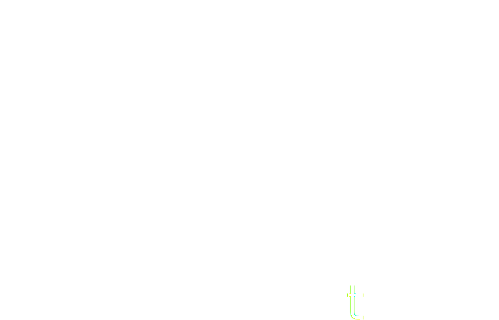
\includegraphics[width=\linewidth]{figures/white_noise.pdf}
    \vfill
    }
\end{column}
\begin{column}{0.33\linewidth}
    \centering
    \vbox to .8\textheight{%
    Memory
    \vfill
    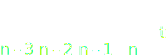
\includegraphics[width=\linewidth]{figures/memory.pdf}
    \vfill
    }
\end{column}
\end{columns}
\note[item]{Explain construction of Wilks' plot}
\note[item]{Stochasticity: capture variability}
\note[item]{Memory: noise values not independent, unresolved tendencies persist
over time, reminiscent of Takens' embedding theorem}
\end{frame}

\begin{frame}{I will ask:}
\begin{itemize}
    \item Do toy model parametrisation methods generalise to real systems?
    \item What level of predictability is achievable if the system has
        \emph{inherent} stochasticity and/or memory?
\end{itemize}
\note[item]{Toy models are good but\dots}
\note[item]{Even if the system is deterministic in principle, there may be
completely unknown degrees of freedom, or we might not have a complete
understanding of the physics}
\end{frame}

\begin{frame}{I will consider 2D \rb{} convection}
\centering
\includegraphics[height=0.5\textheight]{figures/rbc.png}
\begin{equation*}
    \left\{ \quad
    \begin{aligned}
        \partial_t \vec{u} + (\vec{u} \cdot \grad) \vec{u}
            &= -\frac{1}{\rho_0} \grad p + \nu \nabla^2 \vec{u}
            + g\alpha (T - T_0) \uvec{z} \\
        \partial_t T + (\vec{u} \cdot \grad) T &=  D_T \nabla^2 T \\
        \grad \cdot \vec{u} &= 0
    \end{aligned}
    \right.
\end{equation*}
\note{Explain boundary conditions and typical steady behaviour}
\end{frame}

\begin{frame}{The equations are decomposed into coarse and fine parts}
\begin{columns}
\begin{column}{0.7\linewidth}
    \centering
    \includestandalone[height=0.85\textheight]{figures/simplegrid}
\end{column}
\begin{column}{0.2\linewidth}
    \begin{align*}
        u &\to \begingroup \color{hilight} \bar{u} \endgroup + u' \\
        w &\to \begingroup \color{hilight} \bar{w} \endgroup + w' \\
        T &\to \begingroup \color{hilight} \bar{T} \endgroup + T'
    \end{align*}
\end{column}
\note{Puts RBC into same form as toy models!}
\begin{column}{0.1\linewidth}

\end{column}
\end{columns}
\end{frame}

\begin{frame}{I will perform the following experiments:}
\begin{enumerate}
    \item<1-> Integrate full coupled system as truth, divide data into training
        and evaluation sets
    \item<2-> Parametrise the model using different schemes:
    \begin{enumerate}
        \item Trivial (i.e., nothing)
        \item Deterministic regression model
        \item Regression + stochasticity
        \item Regression + stochasticity + memory (e.g., autoregressive)
        \item More advanced methods in literature
    \end{enumerate}
    \item<3-> Repeat (1-2) when the ``truth'' system has inherent:
    \begin{enumerate}
        \item Stochastic forcing
        \item Memory
        \item Both of the above
    \end{enumerate}
\end{enumerate}
\end{frame}

\begin{frame}{Parametrisation performance will be assessed by:}
\begin{itemize}
    \item Short-term forecast accuracy:
    \begin{itemize}
        \item RMSE
    \end{itemize}
    \item Long-term average ``climate'' prediction:
    \begin{itemize}
        \item Statistical moments of the coarse variables (mean, variance,
            skewness, etc.)
        \item Closeness of their PDFs (e.g., Kolmogorov-Smirnov statistic)
    \end{itemize}
\end{itemize}
\end{frame}

\begin{frame}{I envision the following outcomes:}
\begin{itemize}
    \item<1> For each parametrisation scheme:
    \begin{itemize}
        \item Quantitative assessment of performance, strengths, weaknesses
        \item Determination of ideal settings
        \item Scalability from toy models to more complex systems
        \item How do these change if the system has inherent
            stochasticity/memory?
    \end{itemize}
    \item<2> Concluding recommendations on scheme choice and settings for
        different modelling objectives (i.e., forecasting vs. climate
        statistics)
    \item<3> Implications for parametrisation development in weather/climate
        models
\end{itemize}
\end{frame}

\end{document}
